\section{The Algorithm}
\label{sec:algorithm}

In this section, we will briefly describe the steps our algorithm takes and then provide more details on key parts of it. The algorithm consists of two parts, a \emph{Compress} function and a \emph{Decompress} function. 

\begin{figure}[tbh]
  \centering
  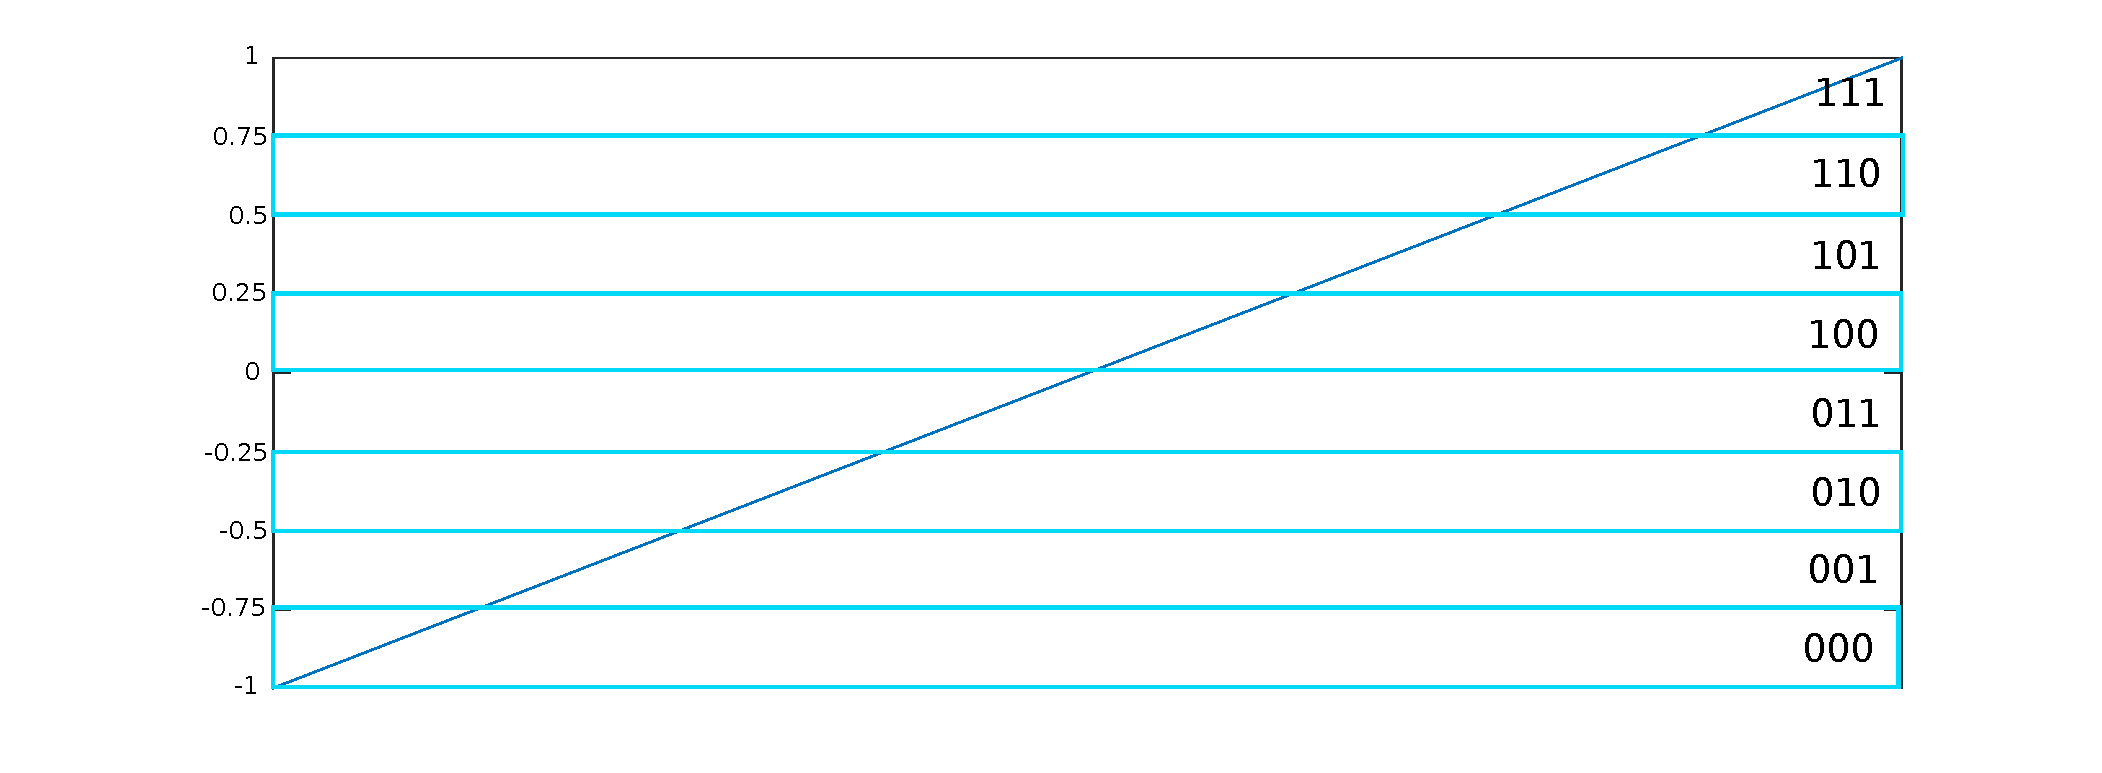
\includegraphics[width=\columnwidth]{images/bqQuantizer}
  \caption{Neural Network Structure for compression.}
  \label{fig:bpQuantizer}
\end{figure}

\subsection{Compression} \label{sec:compress}
In the Compress function, to which one passes the original image as an argument, the following steps are completed:
\begin{enumerate}
\item \emph{Feature extraction}. First, we add rows and columns to the image matrix so that the number of rows and columns is evenly divisible by 8, the predefined patch size. We then extract patches of size \(8 \times~8\) and return them as a single column vector.

\item \emph{Conversion}. We convert the image data, consisting of pixels with values between 0 and 255, to real values in the range \([-1, 1]\). 

\item \emph{Training}. As described in \ref{sec:trainfcn}, training is performed ``globally''. If one wants to do additional local training, we include a set of 100 to 300 randomly chosen column vectors of the current image in the training.

\item \emph{Network separation}. After the training is done, we separate the neural network into two parts, one including input and hidden layer and the other including hidden and output layer. The first will be our compression network, using the values of the hidden layer as the output, while the latter is the decompression network, taking the values of the hidden layer as input and returning an approximation of the original data.

\item \emph{Network encoding} is done by applying the compression network to the column vectors of the image, effectively reducing data size.

\item \emph{Quantization} as shown in Figure~\ref{fig:bpQuantizer} is the process of mapping a large set of values in a partitioned interval to the set of integers \(\{1,\dots,k\}\). After compression, we quantize the output using 4 bits for quantization levels, leaving us with 16 identically wide intervals. After mapping the compression output to these values, we store two indices per byte.

\item \emph{Transmission}. The final data structure of the compressed image consists of the compressed and quantized output, the decoding net, image size and the parameters patch size, hidden layer node count and quantization bits.
\end{enumerate}

\subsection{Decompression} \label{sec:decompression}
The decompression works basically by reversing the compression steps:
\begin{enumerate}
\item \emph{Dequantization} is the process of mapping the integer values back to the real values of the particular intervals. 

\item \emph{Neural net decoding} is done using the right part of the neural network, the decoding net, and applying it to the dequantized data.

\item \emph{Conversion} from real values in the interval \([-1, 1]\) to pixel values.

\item \emph{Reassemble} the extracted subimages into one image. In this function, we take the individual column vectors, reshape them into image patches, and put them into the right spot in the original sized image matrix. 
\end{enumerate}

